\documentclass[11pt]{article}

\usepackage{fancyhdr}
\usepackage{geometry}
\usepackage{graphicx}
\graphicspath{{images/}}

%margin
 \geometry{
 left=25mm,
 right=25mm,
 top=25mm,
 bottom=25mm,
 }

\pagestyle{fancy}
%\renewcommand{\headrulewidth}{0pt}
\lhead{Hadoop - Content based Search \& Retrieval}
\rhead{Divide and Conquer Strategies}

\begin{document}

\noindent
\textbf{
	\large Assignment No 3 \\ \\
} 

\textbf{
	 Aim​:} Use of divide and conquer strategies to exploit distributed/parallel/concurrent processing of the  above  to identify objects, morphisms, overloading in functions (if any), and functional relations and any other  dependencies (as per requirements).  \\ \\ \\

\noindent
\textbf{Divide and conquer} \\ \\
Divide and Conquer (D\&C) is an algorithm design paradigm based on multi­branched recursion.  A typical Divide and Conquer algorithm solves a problem using following three steps. \\ \\
1. Divide: Break the given problem into subproblems of same type. \\
2. Conquer: Recursively solve these subproblems \\
3. Combine: Appropriately combine the answers  The solutions to the sub­problems are then combined to give a solution to the original problem. \\ \\ \\

\textbf{Demonstration:} \\ \\

\itemize{
\item Divide: Divide the search by mapping the input by using mappers of Map Reduce.
\item Conquer: Reduce the number of search by aggregation.
\item Combine: Combine the relevant searches as per the keywords entered.
}

\newpage

\large \textbf{Divide and Conquer} \\ \\ \\ \\
\begin{figure}[h]
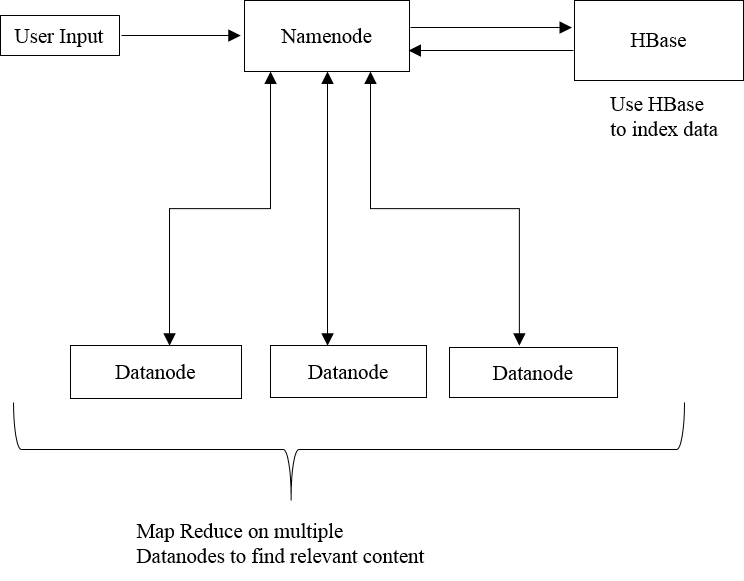
\includegraphics{divide_and_conquer}
\end{figure}

\end{document}